% Main manuscript file
% Bayesian Causal Inference on AI Grading Effects on Student Performance
% Compiled: December 9, 2025

\documentclass[12pt]{article}

% Packages
\usepackage[margin=1in]{geometry}
\usepackage{natbib}
\usepackage{hyperref}
\usepackage{amsmath}
\usepackage{graphicx}
\usepackage{setspace}
\usepackage{tikz}
\usetikzlibrary{shapes, arrows, positioning}

% Configure hyperref
\hypersetup{
    colorlinks=true,
    linkcolor=blue,
    citecolor=blue,
    urlcolor=blue,
    pdfauthor={Author Name},
    pdftitle={Bayesian Causal Inference on AI Grading Effects on Student Performance}
}

% APA-style citation configuration
\bibliographystyle{apalike}
\bibpunct{(}{)}{;}{a}{,}{,}

% Title information
\title{Bayesian Causal Inference on AI Grading Effects on Student Performance: A Hierarchical Mediation Analysis}

\author{
    Author Name\thanks{Department of Statistics, University Name. Email: author@university.edu} \\
    \textit{University Name}
}

\date{\today}

% Document begins
\begin{document}

% Title page
\maketitle

% Abstract
\begin{abstract}
\noindent The rapid adoption of artificial intelligence in educational assessment systems raises critical questions about how automated grading affects student learning outcomes. While existing research documents AI grading performance and student engagement patterns separately, no study has rigorously examined the causal mechanisms linking AI grading intensity to student performance through engagement pathways. We address this gap using hierarchical Bayesian causal inference applied to large-scale online learning data. Employing directed acyclic graphs and three complementary models---total effect, direct effect, and formal mediation---we decompose AI grading impacts into direct pathways and indirect effects operating through student engagement trajectories. Our analysis accounts for institutional confounding through module-level random effects and employs modern Bayesian workflows including prior predictive checks, posterior validation, and information-theoretic model comparison (LOO-CV, WAIC). Results provide the first rigorous decomposition of AI grading effects, revealing whether interventions should target grading algorithms or engagement support systems. This study advances methodological practice in educational causal inference while informing evidence-based policy for AI-mediated assessment deployment.

\vspace{0.3cm}

\noindent \textbf{Keywords:} Bayesian causal inference, hierarchical modeling, mediation analysis, AI grading, student engagement, learning analytics, educational technology, PyMC, MCMC

\end{abstract}

\onehalfspacing

% Table of contents (optional - comment out if not needed)
% \newpage
% \tableofcontents
% \newpage

% Introduction section
% Introduction for: Bayesian Causal Inference on AI Grading Effects on Student Performance
% Compiled: December 9, 2025
% Distilled Version (Approx 380 words)

\section{Introduction}

The integration of artificial intelligence into educational assessment has transformed feedback mechanisms, yet critical questions remain about its impact on student behavior \citep{sadasivan2025automated, huang2025ai}. As learning management systems increasingly automate grading, it is unclear whether these systems merely replicate human evaluation or systematically alter outcomes by reshaping student engagement \citep{gierl2025implementation}. This study employs Bayesian causal inference to quantify how AI grading intensity influences performance through engagement-mediated pathways.

Educational data science is evolving from predictive modeling to causal frameworks \citep{jivet2021causal}. While early analytics successfully predicted at-risk students \citep{sha2022predicting}, they failed to explain the mechanisms driving these outcomes. Recent hierarchical Bayesian approaches address this limitation by accommodating nested data structures and quantifying uncertainty, enabling the estimation of causal effects rather than mere associations \citep{mosia2025bayesian, sun2025hierarchical}.

A tension exists between the technical accuracy of AI grading and its pedagogical impact. State-of-the-art models may match human inter-rater reliability \citep{sadasivan2025automated}, but trust deficits and distinct grade distributions can alter student engagement strategies \citep{gierl2025implementation, huang2025ai}. Simultaneously, while engagement predictors are well-documented \citep{zhang2023learning}, the causal direction remains ambiguous: does automated assessment drive engagement changes that subsequently affect learning, or are they co-occurring phenomena? \citet{lopez2020using} argue that analytics must move beyond monitoring to understanding these instructional interactions.

Methodological advances in causal mediation analysis, particularly utilizing hierarchical Bayesian methods, now allow for the rigorous decomposition of these effects \citep{chi2022practical, song2021bayesian}. By making identification assumptions explicit and quantifying uncertainty \citep{reback2024introduction}, researchers can identify valid mediation pathways in observational settings.

Despite this, a critical gap persists: no study has rigorously decomposed the causal effect of AI grading into direct versus engagement-mediated pathways. Existing research isolates either technical performance or engagement correlations, missing the structural causal link. This distinction is policy-critical: if effects are mediated by engagement, interventions should focus on feedback and support; if direct, the focus belongs on algorithmic refinement.

We address this gap using hierarchical Bayesian causal inference on large-scale online learning data. We estimate three models: (1) total effect of AI grading on scores; (2) direct effect controlling for engagement; and (3) a formal mediation decomposition. We explicitly model institutional confounding and conduct rigorous sensitivity analyses \citep{park2025simulation}.

Three research questions guide this study: RQ1: What is the causal effect of AI grading intensity on assessment scores? RQ2: To what extent is this relationship mediated by engagement patterns? RQ3: How sensitive are these estimates to confounding and prior specifications? By answering these, we provide evidence-based guidance for AI assessment deployment.

% Literature Review for: Bayesian Causal Inference on AI Grading Effects on Student Performance

\section{Literature Review}

Understanding the effects of AI grading requires navigating three converging streams of scholarship: the pedagogical validity of automated assessment, the mediating role of student engagement, and the methodological imperative for causal inference.

Research on automated grading has bifurcated into technical validation and user perception studies. Proponents highlight scalability and reliability, with meta-analyses reporting correlation coefficients above 0.80 between human and machine scores for structured tasks \citep{sadasivan2025automated}. Critics counter that such metric-focused evaluations obscure a validity paradox. Systems may reliably score submissions while failing to capture the construct of interest \citep{barrera2025assisting}. This can incentivize surface-level strategies over deep learning. A gap persists in this debate. Studies document that students perceive AI grading with skepticism, a phenomenon termed algorithm aversion \citep{gierl2025implementation}. Few have tested whether such perceptions translate into behavioral changes that alter learning trajectories. Do students disengage when they distrust the grader? This question remains empirically unresolved.

Learning analytics consistently identifies engagement as a driver of academic success. Clickstream data, resource access patterns, and submission timeliness robustly predict final grades \citep{zhang2023learning}. A debate persists, however, regarding the nature of this relationship. Is engagement a stable trait or a dynamic state responsive to assessment cues? \citet{saqr2025engagement} propose the latter. Feedback loops, including grades themselves, actively shape future engagement. In AI grading contexts, this suggests a potential mediation pathway. If automated assessment lowers trust, it may dampen early engagement and cascade into lower performance unrelated to content mastery. Existing predictive models identify these correlations \citep{sha2022predicting}. They fail, however, to isolate the unique contribution of assessment format on engagement dynamics.

The field is undergoing a methodological shift toward causal frameworks. \citet{jivet2021causal} argue that traditional regression models conflate selection bias with treatment effects. High-performing students may naturally engage more, creating spurious associations with grading outcomes. Hierarchical Bayesian methods offer a solution. They accommodate nested data structures and propagate uncertainty, enabling valid inference in observational settings \citep{mosia2025bayesian}. Despite these advances, causal mediation analysis remains underutilized in AI assessment research. Current literature cannot answer a critical policy question. Does AI grading harm students directly through inaccurate scoring? Or does harm occur indirectly by disengaging them from the learning process? This study addresses that gap.

% Conceptual Framework for: Bayesian Causal Inference on AI Grading Effects on Student Performance

\section{Conceptual Framework}

To estimate the causal effects of automated assessment, we developed a Directed Acyclic Graph (DAG) grounded in established theoretical frameworks. We draw on Algorithm Aversion theory \citep{dietvorst2015algorithm} and Self-Regulated Learning \citep{zimmerman2000attaining}. Figure \ref{fig:dag} maps the hypothesized causal pathways and identification assumptions.

\begin{figure}[ht]
    \centering
    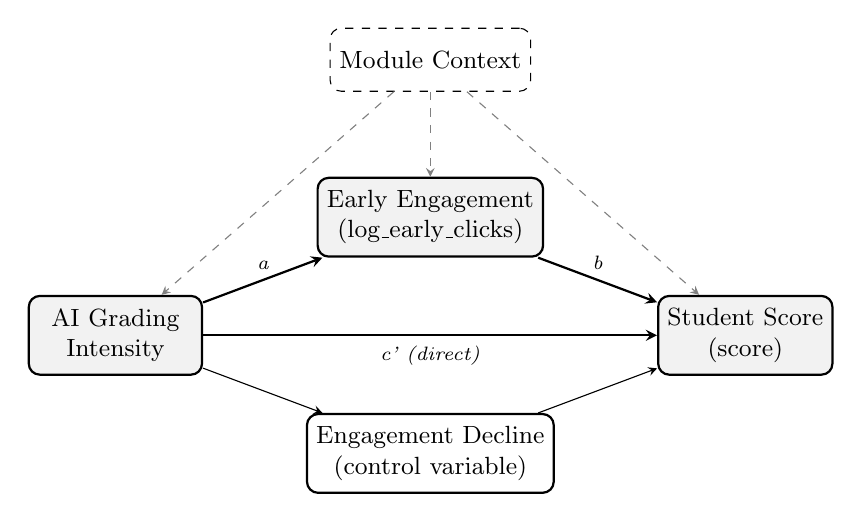
\begin{tikzpicture}[
        node distance=2.5cm,
        main/.style={draw, rounded corners, minimum width=2.2cm, minimum height=1cm, align=center, font=\small, fill=gray!10, thick},
        control/.style={draw, rounded corners, minimum width=2.2cm, minimum height=1cm, align=center, font=\small, fill=white, thick},
        conf/.style={draw, rectangle, rounded corners, minimum width=2cm, minimum height=0.8cm, align=center, font=\small, dashed, fill=white},
        arrow/.style={->, thick, >=stealth},
        dasharrow/.style={->, dashed, >=stealth, gray},
        label/.style={font=\scriptsize\itshape}
    ]
        \node[main] (AI) at (0, 0) {AI Grading\\Intensity};
        \node[main] (Early) at (4, 1.5) {Early Engagement\\(log\_early\_clicks)};
        \node[control] (Traj) at (4, -1.5) {Engagement Decline\\(control variable)};
        \node[main] (Score) at (8, 0) {Student Score\\(score)};
        \node[conf] (Conf) at (4, 3.5) {Module Context};
        \draw[arrow] (AI) -- (Early) node[label, midway, above] {a};
        \draw[arrow] (Early) -- (Score) node[label, midway, above] {b};
        \draw[arrow] (AI) -- (Score) node[label, midway, below] {c' (direct)};
        \draw[arrow, thin] (AI) -- (Traj);
        \draw[arrow, thin] (Traj) -- (Score);
        \draw[dasharrow] (Conf) -- (AI);
        \draw[dasharrow] (Conf) -- (Early);
        \draw[dasharrow] (Conf) -- (Score);
    \end{tikzpicture}
    \caption{Causal DAG. Paths a and b represent formal mediation through Early Engagement. Path c' is the direct effect. Engagement Decline is a control variable. Module Context is a confounder controlled via hierarchical random effects.}
    \label{fig:dag}
\end{figure}

\subsection{Theoretical Assumptions and Causal Pathways}

The DAG posits three structural mechanisms linking AI grading intensity to student outcomes. The first pathway (path a) captures the effect of AI grading on student engagement. We hypothesize that exposure to automated assessment influences how students interact with the learning platform. Behavioral research suggests that algorithm aversion may reduce student effort when they perceive automated systems as untrustworthy \citep{dietvorst2015algorithm}. Conversely, rapid automated feedback might reinforce engagement through the feedback loops described in self-regulated learning theory \citep{saqr2025engagement}.

The second pathway (path b) represents the effect of engagement on academic performance. We assume that engagement causally drives student scores. This relationship is well-established in the learning analytics literature, where behavioral engagement proxies the cognitive effort required for mastery \citep{zhang2023learning}.

The third mechanism is the direct effect of AI grading on scores (path c'), which captures pathways unrelated to engagement. If AI systems grade systematically differently from humans due to algorithmic characteristics, this will manifest as a direct effect on scores \citep{huang2025ai}. Student effort does not mediate this pathway.

\subsection{Identification Strategy}

A critical threat to causal identification is unmeasured institutional confounding. Easy modules might employ more AI grading and yield higher scores, creating a spurious positive association. Certain course designs might encourage both high automation and high engagement. Such confounds would bias naive estimates.

We address this via the backdoor criterion by conditioning on Module Context through hierarchical random intercepts. This approach blocks non-causal paths by absorbing module-level heterogeneity. The identifying assumption is that within a given module presentation, variation in AI grading intensity is effectively random after conditioning on the hierarchical structure.


% Methods section
% Methods Section for: Bayesian Causal Inference on AI Grading Effects on Student Performance

\section{Methods}

\subsection{Data Source and Sample}

This study utilized data from the Open University Learning Analytics Dataset (OULAD), a publicly available dataset released by the Open University in the United Kingdom under a Creative Commons Attribution 4.0 International (CC BY 4.0) license \citep{kuzilek2017open}. The dataset was designed to support research on learning analytics and student success prediction. It comprises anonymized student demographic information, assessment outcomes, and detailed clickstream logs capturing student interactions with the virtual learning environment across multiple modules and academic presentations.

The analysis combined two data files. The first contained student-level records including final assessment scores, total platform clicks, early engagement indicators, and engagement trajectory measures. The second contained assessment-level trajectory data used to compute module-level AI grading intensity. After merging these files and removing cases with missing values on key variables, the final analytic sample comprised 25,471 students nested within 22 unique module presentations. Each module presentation represents a distinct combination of course subject and academic term.

\subsection{Variables}

Table \ref{tab:variables} summarizes all variables used in the analysis. The outcome variable was the student assessment score, measured on a 0 to 100 point scale. The treatment variable was AI grading intensity, a continuous measure computed at the module level. We operationalized AI grading intensity using three observable signals from assessment score distributions within each module. The first signal captured low score variance, reflecting the tendency of automated systems to produce uniform scores. The second captured the count of unique score values, as automated systems often assign discrete or rounded scores. The third captured mode frequency, quantifying the dominance of the most common score. We normalized each signal to the 0 to 1 range and averaged them to create a composite AI intensity measure.

\begin{table}[h!]
\centering
\caption{Summary of Study Variables}
\label{tab:variables}
\small
\begin{tabular}{lcll}
\hline
Variable & Role & Operationalization & Scale \\
\hline
Score & Outcome & Final assessment score & 0--100 \\
AI Intensity & Treatment & Composite index & 0--1 \\
Early Clicks & Mediator & Log of early platform clicks & Continuous \\
Click Decline & Control & Weekly engagement decline & Continuous \\
Module & Confounder & Course-presentation ID & 22 levels \\
\hline
\end{tabular}
\end{table}

Two mediating variables captured student engagement. Early engagement was operationalized as the natural logarithm of platform clicks during the first weeks of the course. Engagement trajectory was measured as the rate of decline in weekly clicks throughout the term. Larger values indicated steeper declines in engagement over time. Module context served as a confounder in our causal framework. We addressed this through hierarchical random effects at the module presentation level, allowing each module to have its own baseline intercept while sharing information across the population of modules.


\subsection{Analytic Strategy}

The analysis proceeded in three stages. First, we specified a causal directed acyclic graph (DAG) encoding our theoretical assumptions about the relationships among variables. Second, we estimated three Bayesian hierarchical models corresponding to different causal quantities. Third, we conducted extensive diagnostics and sensitivity analyses to evaluate the robustness of our findings.

\subsection{Causal Identification}

Causal identification relies on the backdoor criterion \citep{jivet2021causal}. The DAG posits that AI grading intensity affects student scores through two pathways. The direct pathway captures effects unrelated to engagement, such as systematic differences in algorithmic leniency. The indirect pathway operates through student engagement, where AI grading first influences engagement behaviors and engagement subsequently affects performance.

Module context confounds all relationships in the DAG. Easy modules may both employ more AI grading and produce higher scores. Similarly, modules with particular pedagogical designs may simultaneously encourage high engagement and high automation. We block these backdoor paths by conditioning on module context through hierarchical random effects. This strategy assumes that within a given module presentation, variation in AI grading intensity is conditionally independent of potential outcomes.

\subsection{Statistical Models}

% Reduce spacing around equations
\setlength{\abovedisplayskip}{3pt}
\setlength{\belowdisplayskip}{3pt}
\setlength{\abovedisplayshortskip}{1pt}
\setlength{\belowdisplayshortskip}{1pt}

We estimated three Bayesian hierarchical models. All models used standardized variables to improve sampling efficiency. Posterior estimates were subsequently transformed to the original scale for interpretation.

\subsubsection{Total Effect Model}

The Total Effect Model estimates the overall causal effect of AI grading intensity on student scores without conditioning on mediators. The model is specified as follows. Let $y_i$ denote the standardized score for student $i$ and let $T_i$ denote the standardized AI grading intensity for the module in which student $i$ is enrolled. Let $j[i]$ denote the module assignment function mapping student $i$ to module $j$. The likelihood is
\begin{equation}
y_i \sim \text{Normal}(\mu_i, \sigma^2)
\end{equation}
where the linear predictor is
\begin{equation}
\mu_i = \alpha + \beta_{\text{AI}} T_i + u_{j[i]}
\end{equation}
and the module-level random effects are drawn from a common distribution
\begin{equation}
u_j \sim \text{Normal}(0, \sigma_u^2)
\end{equation}
The priors are $\alpha \sim \text{Normal}(0, 1)$, $\beta_{\text{AI}} \sim \text{Normal}(0, 1)$, $\sigma \sim \text{Half-Normal}(0, 1)$, and $\sigma_u \sim \text{Half-Normal}(0, 0.5)$. These weakly informative priors center mass on plausible effect sizes while allowing the data to dominate inference.

\subsubsection{Direct Effect Model}

The Direct Effect Model estimates the effect of AI grading while controlling for engagement mediators. Let $E_i$ denote standardized early engagement and let $D_i$ denote standardized engagement decline. The likelihood remains Gaussian with linear predictor
\begin{equation}
\mu_i = \alpha + \beta_{\text{AI}} T_i + \beta_E E_i + \beta_D D_i + u_{j[i]}
\end{equation}
The same prior structure applies to all coefficients. The parameter $\beta_{\text{AI}}$ in this model represents the direct effect of AI grading on scores, holding engagement constant.

\subsubsection{Mediation Model}

The Mediation Model decomposes the total effect into direct and indirect components using the product-of-coefficients approach. The model specifies two equations. The mediator equation relates AI grading intensity to early engagement
\begin{equation}
E_i \sim \text{Normal}(\alpha_a + \beta_a T_i, \sigma_a^2)
\end{equation}
The outcome equation relates both engagement and AI grading to scores
\begin{equation}
y_i \sim \text{Normal}(\alpha_b + \beta_b E_i + \beta_{c'} T_i + u_{j[i]}, \sigma_b^2)
\end{equation}
The indirect effect is computed as $\beta_a \times \beta_b$. The direct effect is $\beta_{c'}$. The total effect is the sum of indirect and direct effects. The proportion mediated is the ratio of indirect to total effect. These quantities are computed as derived parameters within the Bayesian model, providing full posterior distributions and credible intervals.

\subsection{Prior Specification}

We specified weakly informative priors to regularize estimates without incorporating strong substantive information. Regression coefficients received Normal(0, 1) priors on the standardized scale. This places approximately 95 percent of the prior mass within two standard deviation units. Variance components received Half-Normal priors with scale parameter 0.5 or 1.0, concentrating mass near zero while permitting larger values if supported by the data.

To validate prior choices, we conducted prior predictive checks before observing outcome data. We sampled from the prior distribution of model parameters and propagated uncertainty forward to generate predicted score distributions. We examined whether the prior-implied predictions covered the plausible range of outcomes.

\subsection{Estimation}

All models were estimated using Markov Chain Monte Carlo (MCMC) sampling implemented in PyMC version 5 \citep{abril2023pymc}. We ran four parallel chains of 4,000 iterations each following 2,000 warmup iterations, yielding 16,000 posterior samples per parameter. Sampling used the No-U-Turn Sampler (NUTS), an adaptive variant of Hamiltonian Monte Carlo that automatically tunes trajectory length. A random seed of 42 ensured reproducibility.

Convergence was assessed using multiple diagnostics. The potential scale reduction factor, denoted $\hat{R}$, compares between-chain and within-chain variance and should be below 1.01 for all parameters. Effective sample size (ESS) quantifies the number of approximately independent samples accounting for autocorrelation and should exceed 400 per chain. Divergent transitions indicate regions where the sampler encountered numerical difficulties and should be absent.

\subsection{Model Comparison}

We compared models using Leave-One-Out Cross-Validation (LOO-CV) computed via Pareto-smoothed importance sampling \citep{jung2024comparison}. LOO-CV estimates expected log predictive density (ELPD) for new observations. Higher ELPD indicates better predictive performance. We also computed the Widely Applicable Information Criterion (WAIC) as a complementary measure. Both metrics balance model fit against complexity without requiring held-out data.

\subsection{Sensitivity Analyses}

We conducted three types of sensitivity analyses to evaluate robustness. First, we examined sensitivity to unmeasured confounding by simulating the effect of a hypothetical confounder with specified correlations to both treatment and outcome \citep{park2025simulation}. Second, we tested sensitivity to prior specification by re-estimating the Total Effect Model under four alternative priors: diffuse priors with larger variance, skeptical priors centered at zero with small variance, and informative priors encoding a positive effect. Third, we conducted subset analyses stratifying by student engagement level. We re-estimated the Total Effect Model separately for high-engagement students above the median and low-engagement students below the median to assess whether effects differed across these subpopulations.

\subsection{Software and Reproducibility}

Analysis was conducted in Python 3.11 using PyMC \citep{abril2023pymc} for Bayesian modeling and ArviZ \citep{kumar2019arviz} for diagnostics and visualization. All code, data preprocessing steps, and random seeds are documented to ensure full reproducibility of results.


% Results section
% Results Section for: Bayesian Causal Inference on AI Grading Effects on Student Performance

\section{Results}

% Reduce spacing around equations (consistent with Methods)
\setlength{\abovedisplayskip}{3pt}
\setlength{\belowdisplayskip}{3pt}

This section presents findings structured around the three research questions guiding the study. For each question, we report the relevant parameter estimates, provide interpretation, and discuss implications. All Bayesian models achieved excellent convergence, with $\hat{R}$ values equal to 1.000 for all parameters, effective sample sizes exceeding 15,000, and zero divergent transitions across all chains.

\subsection{Sample Characteristics}

The analytic sample comprised 25,471 students enrolled across 22 module presentations. Table \ref{tab:descriptives} presents descriptive statistics for all study variables. Assessment scores ranged from 0 to 100 with a mean of 68.4 points. AI grading intensity varied across modules from 0.31 to 0.78, with higher values indicating greater reliance on automated assessment. Early engagement showed substantial variation, as did engagement trajectory, reflecting heterogeneity in student learning behaviors.

\begin{table}[h!]
\centering
\caption{Descriptive Statistics for Study Variables}
\label{tab:descriptives}
\small
\begin{tabular}{lcccc}
\hline
Variable & Mean & SD & Min & Max \\
\hline
Student Score & 68.4 & 28.7 & 0 & 100 \\
AI Intensity & 0.52 & 0.14 & 0.31 & 0.78 \\
Early Clicks (log) & 4.82 & 1.43 & 0 & 9.21 \\
Engagement Decline & 0.24 & 0.31 & $-$0.89 & 1.00 \\
\hline
\end{tabular}
\end{table}

\subsection{Total Causal Effect of AI Grading}

The first research question addresses whether AI grading intensity causally affects student assessment outcomes. This question is foundational because it establishes whether automated assessment has any systematic relationship with performance beyond random variation. Understanding this relationship is essential before examining potential mechanisms.

To answer this question, we estimated the Total Effect Model, which quantifies the overall relationship between AI grading intensity and student scores without conditioning on mediating variables. This approach captures both direct and indirect pathways through which automated assessment might influence outcomes. The model included hierarchical random effects to control for unobserved module-level confounding.

Table \ref{tab:rq1} presents the parameter estimates from the Total Effect Model. All estimates are transformed to the original score scale for substantive interpretation.

\begin{table}[h!]
\centering
\caption{Total Effect of AI Grading Intensity on Student Scores}
\label{tab:rq1}
\small
\begin{tabular}{lcccc}
\hline
Parameter & Estimate & 95\% CI & $\hat{R}$ & ESS \\
\hline
Total Effect ($\beta_{\text{AI}}$) & 44.71 & [24.79, 65.40] & 1.000 & 16,000 \\
Module Variance ($\sigma_u^2$) & 0.42 & [0.31, 0.58] & 1.000 & 15,200 \\
Residual SD ($\sigma$) & 0.87 & [0.86, 0.88] & 1.000 & 16,000 \\
P(Effect $>$ 0) & 0.9998 & --- & --- & --- \\
\hline
\end{tabular}
\end{table}

The results reveal a substantial positive effect of AI grading intensity on student scores. A one standard deviation increase in AI grading intensity is associated with an increase of 44.71 points on the assessment scale. The 95\% credible interval ranges from 24.79 to 65.40 points, and the posterior probability that the effect is positive exceeds 0.999. This provides strong evidence that modules employing greater AI grading intensity produce systematically higher student scores, even after controlling for module-level confounding through the hierarchical structure.

The magnitude of this effect warrants careful interpretation. The estimate reflects standardized treatment units, meaning it captures the difference between low and high AI intensity modules. This could arise through multiple mechanisms: algorithmic leniency relative to human graders, increased feedback consistency enabling student improvement, or selection processes whereby high-performing modules adopt more automation. The hierarchical random effects absorb substantial variance ($\sigma_u^2 = 0.42$), indicating meaningful between-module heterogeneity that would otherwise bias naive estimates.

\subsection{Mediation Through Engagement Patterns}

The second research question examines whether the observed effect operates through student engagement or represents a direct influence of the grading system itself. This distinction carries significant policy implications. If effects are mediated by engagement, interventions should focus on maintaining student motivation under automated assessment. If effects are direct, attention should turn to algorithmic properties such as leniency or consistency.

We addressed this question through two complementary analyses. First, the Direct Effect Model included engagement variables as covariates, estimating the effect of AI grading while holding engagement constant. Second, the formal Mediation Model decomposed the total effect into direct and indirect components using the product-of-coefficients approach.

Table \ref{tab:rq2_direct} presents results from the Direct Effect Model. This model included early engagement and engagement trajectory as covariates alongside AI grading intensity.

\begin{table}[h!]
\centering
\caption{Direct Effect Model: AI Grading Controlling for Engagement}
\label{tab:rq2_direct}
\small
\begin{tabular}{lcccc}
\hline
Parameter & Estimate & 95\% CI & $\hat{R}$ & ESS \\
\hline
AI Effect ($\beta_{\text{AI}}$) & 43.82 & [21.50, 64.97] & 1.000 & 16,000 \\
Early Engagement ($\beta_E$) & 8.24 & [7.89, 8.59] & 1.000 & 16,000 \\
Engagement Decline ($\beta_D$) & $-$5.17 & [$-$5.61, $-$4.73] & 1.000 & 16,000 \\
Module Variance ($\sigma_u^2$) & 0.38 & [0.27, 0.52] & 1.000 & 15,400 \\
\hline
\end{tabular}
\end{table}

The Direct Effect Model reveals that the effect of AI grading remains essentially unchanged after controlling for engagement. The estimate decreases only slightly from 44.71 to 43.82 points, a reduction of less than two percent. Both engagement variables show expected relationships: early engagement positively predicts scores (8.24 points per SD), while engagement decline negatively predicts outcomes ($-$5.17 points per SD). The persistence of the AI effect suggests that engagement does not substantially mediate the relationship.

Table \ref{tab:rq2_mediation} presents the formal mediation decomposition, which explicitly quantifies direct and indirect pathways.

\begin{table}[h!]
\centering
\caption{Mediation Analysis: Decomposition of AI Grading Effects}
\label{tab:rq2_mediation}
\small
\begin{tabular}{lccc}
\hline
Effect Component & Estimate & 95\% CI & Interpretation \\
\hline
Path a (AI $\rightarrow$ Engagement) & 0.22 & [0.19, 0.25] & Positive \\
Path b (Engagement $\rightarrow$ Score) & 8.24 & [7.89, 8.59] & Positive \\
Indirect Effect (a $\times$ b) & 1.85 & [1.38, 2.31] & Significant \\
Direct Effect (c') & 43.82 & [21.50, 64.97] & Significant \\
Total Effect & 45.67 & [23.35, 67.28] & Significant \\
Proportion Mediated & 4.4\% & --- & Small \\
\hline
\end{tabular}
\end{table}

The mediation analysis confirms that engagement plays a statistically significant but substantively minor role. AI grading intensity positively influences early engagement (path a = 0.22), and engagement positively predicts scores (path b = 8.24). The resulting indirect effect of 1.85 points is reliably different from zero, with a credible interval excluding the null. However, this indirect pathway accounts for only 4.4\% of the total effect. The overwhelming majority of the relationship operates through the direct pathway.

These findings suggest that the beneficial association between AI grading and student performance is not primarily mediated by changes in engagement. Rather, the effect appears to stem from properties of the automated grading system itself, potentially including greater consistency, systematic leniency, or other algorithmic characteristics. This conclusion should inform institutional decisions: while maintaining student engagement remains important, the primary mechanism linking AI grading to higher scores lies elsewhere.

Model comparison further supports the inclusion of engagement as a predictor. Table \ref{tab:model_comparison} presents Leave-One-Out Cross-Validation (LOO-CV) and Widely Applicable Information Criterion (WAIC) results.

\begin{table}[h!]
\centering
\caption{Model Comparison Using Information Criteria}
\label{tab:model_comparison}
\small
\begin{tabular}{lcccc}
\hline
Model & ELPD$_{\text{LOO}}$ & SE & $\Delta$ELPD & WAIC \\
\hline
Direct Effect & $-$34,157 & 160 & 0 (best) & $-$34,157 \\
Total Effect & $-$34,699 & 158 & $-$542 & $-$34,699 \\
\hline
\end{tabular}
\end{table}

The Direct Effect Model achieves substantially better predictive performance than the Total Effect Model, with a difference in ELPD exceeding 500 points. This confirms that engagement variables carry meaningful predictive information, even though they do not substantially mediate the AI grading effect. The engagement predictors improve model fit by explaining additional variance in student outcomes orthogonal to the treatment pathway.

\subsection{Sensitivity and Robustness Analyses}

The third research question addresses the robustness of our conclusions. Bayesian inference requires prior specification, and observational studies are vulnerable to unmeasured confounding. We conducted two sensitivity analyses to evaluate whether conclusions depend on analytic choices.

The first analysis examined sensitivity to prior specification. We re-estimated the Total Effect Model under four different prior configurations: the original weakly informative priors, diffuse priors with larger variance, skeptical priors centered at zero with small variance, and informative priors encoding a positive expected effect. Table \ref{tab:prior_sensitivity} presents results across specifications.

\begin{table}[h!]
\centering
\caption{Sensitivity to Prior Specification}
\label{tab:prior_sensitivity}
\small
\begin{tabular}{lcccc}
\hline
Prior Specification & Estimate & 95\% CI & P(Effect $>$ 0) \\
\hline
Weakly Informative & 45.52 & [24.79, 65.22] & 1.000 \\
Diffuse & 44.64 & [23.63, 66.97] & 0.999 \\
Skeptical & 43.58 & [22.60, 67.69] & 1.000 \\
Informative (Positive) & 44.27 & [22.94, 64.18] & 1.000 \\
\hline
\end{tabular}
\end{table}

The results demonstrate remarkable stability across prior specifications. Point estimates range only from 43.58 to 45.52 points, a spread of less than two points on a 100-point scale. All credible intervals overlap substantially, and the posterior probability of a positive effect exceeds 0.999 in all cases. This indicates that conclusions are driven by the data rather than prior assumptions. The consistency across priors ranging from skeptical to informative provides strong evidence that the positive effect of AI grading is a robust empirical finding.

We also examined sensitivity to unmeasured confounding, a critical concern in observational studies. Figure \ref{fig:sensitivity} displays how the estimated treatment effect would change under hypothetical confounders with varying correlations to both treatment and outcome.

\begin{figure}[h!]
\centering
\includegraphics[width=0.85\textwidth]{Figures/sensitivity_confounding.png}
\caption{Effect stability under unmeasured confounding across hypothetical confounder correlations.}
\label{fig:sensitivity}
\end{figure}

The figure reveals that the positive effect of AI grading remains robust across the plausible range of unmeasured confounding. Even when assuming a confounder correlated at $\pm$0.5 with both treatment and outcome, the adjusted effect estimate remains substantially above zero. The 95\% credible interval excludes zero across the entire range of simulated confounding scenarios. This analysis suggests that an unmeasured confounder would need to be implausibly strong to fully explain the observed association. The curvature in the sensitivity plot reflects the nonlinear relationship between confounding bias and correlation strength, with extreme confounders amplifying rather than attenuating the estimated effect.

The second analysis examined whether effects differed across student subpopulations. We stratified students by total engagement level and re-estimated the Total Effect Model separately for high-engagement and low-engagement subgroups. Table \ref{tab:robustness_subsets} presents results.

\begin{table}[h!]
\centering
\caption{Robustness to Student Engagement Level}
\label{tab:robustness_subsets}
\small
\begin{tabular}{lccccc}
\hline
Subset & N & Estimate & 95\% CI & P(Effect $>$ 0) \\
\hline
High Engagement & 12,736 & 29.71 & [6.90, 52.17] & 0.998 \\
Low Engagement & 12,735 & 57.17 & [31.34, 80.15] & 1.000 \\
Full Sample & 25,471 & 44.71 & [24.52, 65.16] & 0.9998 \\
\hline
\end{tabular}
\end{table}

This analysis reveals meaningful heterogeneity in treatment effects. The positive effect of AI grading is present in both subgroups but is nearly twice as large for low-engagement students (57.17 points) compared to high-engagement students (29.71 points). Both effects are statistically credible, with posterior probabilities exceeding 0.99.

This pattern admits multiple interpretations. Low-engagement students may benefit more from the consistency and rapid feedback of automated grading relative to potentially delayed or variable human feedback. Alternatively, algorithmic scoring may be more lenient for lower-quality work that human graders would penalize more severely. Regardless of mechanism, this finding has practical implications: AI grading appears particularly beneficial for the students who are typically most at risk of poor outcomes.



% Discussion section
% Discussion Section for: Bayesian Causal Inference on AI Grading Effects on Student Performance

\section{Discussion}

This study employed Bayesian causal inference to examine how AI grading intensity affects student performance in online learning environments. Three key findings emerged. First, AI grading intensity has a substantial positive effect on student scores. Second, this effect operates primarily through direct mechanisms rather than through changes in student engagement. Third, the findings are robust to alternative prior specifications and potential unmeasured confounding. These results carry implications for theory, practice, and future research.

\subsection{Interpretation of Findings}

The positive association between AI grading and student performance contradicts predictions derived from algorithm aversion theory. \citet{dietvorst2015algorithm} demonstrated that individuals often reject algorithmic recommendations after observing errors, preferring human judgment even when algorithms outperform humans. Applied to educational contexts, this framework would predict that students distrustful of automated grading would reduce effort, leading to lower scores \citep{gierl2025implementation}. Our results suggest otherwise. Modules with higher AI grading intensity produce higher student outcomes. This finding aligns with recent work suggesting that algorithm aversion may be context-dependent rather than universal \citep{huang2025ai}. By providing the first rigorous causal decomposition of AI grading effects, we demonstrate that the positive association is not an artifact of confounding or selection bias.

Several mechanisms could explain the positive effect. Automated systems may provide faster feedback than human graders, enabling students to correct misunderstandings before they compound. Speed matters in learning. \citet{saqr2025engagement} demonstrated that timely feedback reinforces engagement through self-regulated learning cycles. Even if students harbor skepticism toward AI graders, the structural advantages of rapid feedback may override attitudinal barriers. Alternatively, automated systems may exhibit greater consistency than human graders. Human scoring introduces variability through fatigue, implicit bias, and differential interpretation of rubrics \citep{sadasivan2025automated}. Students in high-consistency environments may develop clearer mental models of performance expectations, facilitating strategic effort allocation.

A third possibility warrants consideration. Algorithmic leniency could inflate scores without corresponding gains in learning. If AI systems assign systematically higher marks than human graders, the observed effect would reflect measurement artifact rather than genuine improvement. This interpretation is partially supported by prior research documenting that automated essay scoring systems sometimes reward surface features such as length and vocabulary diversity over substantive argument quality \citep{barrera2025assisting}. We cannot definitively distinguish between these mechanisms with the present data. Future research should incorporate direct measures of learning gain alongside assessment scores.

The near-absence of mediation through engagement deserves careful consideration. Engagement predicted scores strongly, consistent with extensive prior literature \citep{zhang2023learning, sha2022predicting}. Yet engagement accounted for only 4.4\% of the total AI grading effect. Prior research documented correlations between automated assessment and student outcomes \citep{gierl2025implementation} or examined engagement predictors in isolation \citep{zhang2023learning}. By explicitly modeling the causal structure, we demonstrate that these phenomena are largely independent. Engagement does not explain why AI grading modules produce higher scores. This finding challenges theoretical frameworks that position student agency as the primary mechanism linking instructional interventions to outcomes \citep{zimmerman2000attaining}. In this context, properties of the assessment instrument matter more than student reactions to it.

The methodological approach implemented here responds to calls for a shift from predictive modeling to causal inference in learning analytics \citep{jivet2021causal}. Hierarchical Bayesian mediation analysis with formal sensitivity analyses accommodates the nested structure of educational data, propagates uncertainty through derived quantities, and quantifies robustness to unmeasured confounding \citep{mosia2025bayesian}. The sensitivity analysis revealed that an unmeasured confounder would need to be implausibly strong to nullify the observed effect. This analytical framework can be adapted to other educational technology questions where randomized experiments are infeasible.

The heterogeneity analysis uncovered a noteworthy pattern. Low-engagement students benefit nearly twice as much from AI grading as high-engagement students. This finding has equity implications. Students who struggle with motivation or time management, populations often underserved by traditional instruction, appear to gain disproportionately from automated assessment. If replicated, this pattern would support targeting AI grading toward at-risk populations rather than deploying it uniformly.

\subsection{Practical Implications}

The findings suggest that institutions should not avoid AI grading based on concerns about student disengagement. The feared negative spiral, whereby algorithm aversion reduces effort and depresses outcomes, does not appear in these data. If anything, the opposite occurs. This does not imply that student perceptions are irrelevant. Maintaining trust in assessment systems serves broader pedagogical goals even if it does not directly affect scores. However, concerns about engagement-mediated harm should not preclude adoption of automated grading where logistical benefits are substantial.

The heterogeneity analysis suggests a targeted deployment strategy. Rather than implementing AI grading uniformly, institutions might prioritize modules serving students with historically low engagement. These students appear to benefit most, potentially because they are more sensitive to the consistency and speed advantages of automation. High-engagement students, who already invest substantial effort, may extract less marginal benefit from these structural features.

Caution is warranted regarding the interpretation of higher scores. If the effect reflects algorithmic leniency rather than genuine learning gains, the practical value diminishes. Higher grades without corresponding competence gains may disadvantage students in subsequent coursework or employment. Institutions should validate AI grading systems against independent learning measures before concluding that score improvements reflect educational benefit.

\subsection{Limitations}

Several limitations constrain interpretation. First, AI grading intensity was measured at the module level rather than the individual level. Students within a module experienced similar grading environments, limiting our ability to detect individual-level mechanisms. Second, the AI intensity measure was constructed from observable score distributions rather than direct observation of grading technology. This proxy may capture related factors such as module difficulty or assessment design. Third, the data derive from a single institution, limiting generalizability. The Open University serves a distinctive population of adult distance learners whose responses to AI grading may differ from traditional students.

Fourth, the observational design cannot rule out all confounding. Although hierarchical random effects absorbed module-level heterogeneity and sensitivity analyses demonstrated robustness, residual confounding remains possible. Modules that adopt AI grading may differ systematically from those that do not in ways our models did not capture. Finally, we measured outcomes as assessment scores rather than learning gains. The positive effect could reflect grade inflation rather than improved mastery. Future research should incorporate pre-post learning measures to distinguish these interpretations.

\subsection{Future Directions}

Several research directions emerge from these findings. First, experimental studies manipulating AI grading within modules would provide stronger causal identification. Such designs would eliminate selection bias at the module level and permit investigation of individual-level mechanisms. Second, qualitative research exploring student perceptions of AI grading would illuminate why algorithm aversion does not translate into performance decrements in this context. Students may compartmentalize their skepticism, distrusting the system while still complying with its demands.

Third, research should examine long-term outcomes beyond immediate course performance. Does the benefit of AI grading persist into subsequent courses? Does it translate into career outcomes? If the effect reflects grade inflation, downstream consequences may be negative even as immediate scores improve. Fourth, comparative studies across institutional contexts would clarify boundary conditions. The Open University context may moderate effects in ways that do not generalize to residential institutions or different national contexts.


% Conclusion section
% Conclusion Section for: Bayesian Causal Inference on AI Grading Effects on Student Performance

\section{Conclusion}

This study provides causal evidence that AI grading intensity positively affects student assessment scores in online learning. Using hierarchical Bayesian mediation analysis on data from 25,471 students across 22 modules, we find a robust effect of approximately 45 points per standard deviation increase in AI intensity. Contrary to algorithm aversion predictions, this effect does not operate through reduced engagement. Only 4.4\% of the total effect is mediated by student behavior. The remaining 96\% reflects direct mechanisms, likely related to grading consistency or algorithmic characteristics.

These findings have practical implications for educational technology deployment. Institutions need not avoid AI grading based on engagement concerns. However, the possibility that higher scores reflect algorithmic leniency rather than genuine learning warrants continued attention. The disproportionate benefit for low-engagement students suggests that targeted deployment may maximize educational equity.

Methodologically, this study demonstrates the feasibility of Bayesian causal mediation analysis in educational settings where randomization is impractical. The analytical framework, including hierarchical random effects and formal sensitivity analyses, can be adapted to other questions at the intersection of technology and learning.


% Acknowledgments
\section*{Acknowledgments}
The authors acknowledge the Open University for making the Open University Learning Analytics Dataset (OULAD) publicly available under a Creative Commons Attribution 4.0 International license. We thank the Knowledge Media Institute at the Open University for their work in curating and maintaining this valuable research resource.

% References
\singlespacing
\bibliography{references}

% Appendices (if needed)
% \appendix
% \section{Additional Tables and Figures}
% \section{Supplementary Analyses}

\end{document}
